\section{Zustandsraumdarstellung (ZRD)}

\textbf{Grundidee:} Differentialgleichung $n.$ Ordnung eines Systems durch ein \textbf{Differentialgleichungssystem} 
von $n$ Gleichungen $1.$ Ordnung darzustellen.


\subsection{Vorteile der Zustandsraumdarstellung}{253-254}

\begin{itemize}
    \item Innere Systemstabilitäten können erkannt werden, die bei der Untersuchung der UTF 
        nicht festgestellt werden können \textrightarrow\ Einblick in den \textbf{inneren Aufbau} eines Systems
    \item Wichtig in der Regelungstechnik
    \item ZRD hat Vorteile bei der \textbf{numerischen} Behandlung von Systemen
    \item Beschreibung durch \textbf{Energiespeicher}, in der Elektrotechnik $L$ und $C$
    \item \textbf{Nur Integratoren} werden verwendet, keine Differentiatoren
\end{itemize}


\subsection{Zustandsraumdarstellung (ZRD) im Zeitbereich}{255}
\label{ZRD Zeitbereich}

\begin{minipage}[c]{0.4\columnwidth}
    \vspace{-0.3cm}
    
    \begin{empheq}[box=\fbox] {align*}
        \underline{\dot{x}}(t) &= \bm{A} \underline{x}(t) + \bm{B} \underline{u}(t) \\
        \underline{y}(t) &= \bm{C} \underline{x}(t) + \bm{D} \underline{u}(t)
    \end{empheq}

    \begin{tabular}{ll@{}}
        $\underline{u}(t)$   & Eingangsvektor ($m$ Zeilen) \\
        $\underline{x}(t)$   & Zustandsvektor ($n$ Zeilen) \\
        $\underline{y}(t)$   & Ausgangsvektor ($k$ Zeilen) \\
    \end{tabular}
\end{minipage}
\hfill
\begin{minipage}[c]{0.58\columnwidth}
    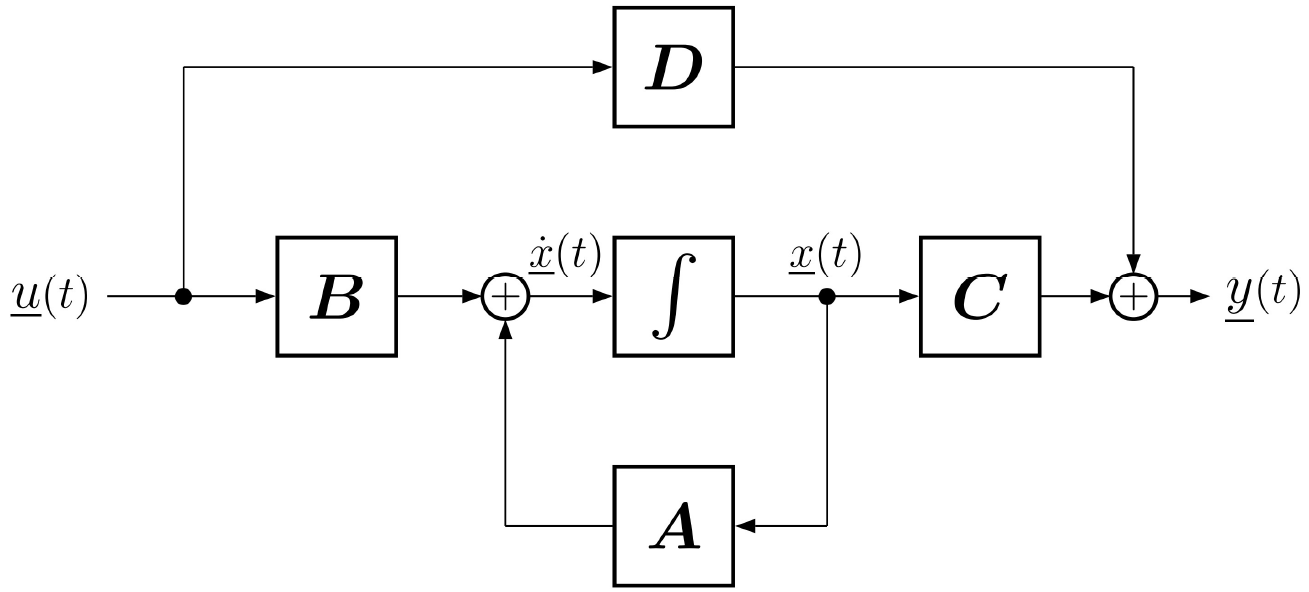
\includegraphics[width=\columnwidth]{images/blockdiagramm_zustandsdarstellung.png}
\end{minipage}


\begin{itemize}
    \item obere Gleichung: \textbf{Zustandsgleichung}
    \item untere Gleichung: \textbf{Ausgangsgleichung}
    \item $\bm{A}$ \textbf{Systemmatrix} ($n \times n$-Matrix) \\
        Sie bestimmt das Verhalten des \textbf{ungestörten Systems} ($\underline{u}(t) = 0$)
        und bestimmt z.B. die innere Stabilität des gesamten Systems.
    \item $\bm{B}$ \textbf{Eingangsmatrix (Steuermatrix)} ($n \times m$-Matrix) \\
        Sie bestimmt die Wirkung der \textbf{Steuergrössen} $\underline{u}(t)$ auf die \textbf{Zustandsgrössen} $\underline{x}(t)$
    \item $\bm{C}$ \textbf{Ausgangsmatrix (Beobachtungsmatrix)} ($k \times n$-Matrix) \\
        Sie kennzeichnet die Abhängigkeit des \textbf{Zustandes} $\underline{x}(t)$ von der beobachtbaren Ausgangsgrösse $\underline{y}(t)$
    \item $\bm{D}$ \textbf{Durchgangsmatrix} ($k \times m$-Matrix) \\
        Sie bestimmt die unmittelbare Wirkung der Eingangsgrösse $\underline{u}(t)$ auf den Ausgang $\underline{y}(t)$
\end{itemize}


\example{ZRD aus Schaltung aufstellen}

\begin{minipage}[c]{0.48\columnwidth}
    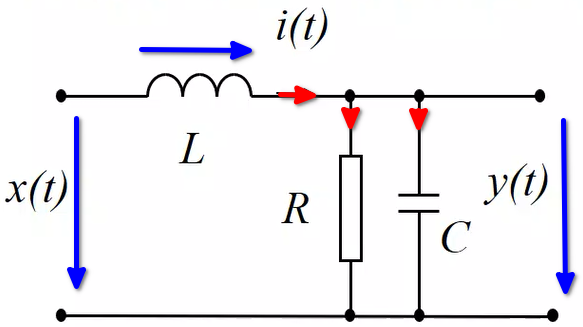
\includegraphics[width=0.9\columnwidth]{images/beispiel_zrd_aus_schaltung.png}
\end{minipage}
\hfill
\begin{minipage}[c]{0.48\columnwidth}
    \begin{itemize}
        \item DGL Induktivität: $\frac{\diff i_L(t)}{\diff t} = \frac{u_L(t)}{L}$ \\
            \textrightarrow\ $u_L(t) = L \cdot \frac{\diff i_L(t)}{\diff t}$
        \item DGL Kapazität: $\frac{\diff u_C(t)}{\diff t} = \frac{i_C(t)}{C}$ \\
        \textrightarrow\ $u_C(t) = \frac{1}{C} \int\limits_{- \infty}^t i(\tau) \, \diff \tau$
    \end{itemize}
\end{minipage}

\begin{minipage}[c]{0.5\columnwidth}
    \begin{empheq}[box=\fbox] {align*}
        \text{Maschen: } & L \cdot \frac{\partial i(t)}{\partial t} + y(t) = x(t) \\
        \text{Knoten: }  & \frac{1}{C} \int\limits_{- \infty}^t \Big( i(\tau) - \frac{y(\tau)}{R} \Big) \, \diff \tau = y(t)
    \end{empheq}
\end{minipage}
\hfill
\begin{minipage}[c]{0.48\columnwidth}
    Beide Gleichungen in ihre differentielle Form bringen (zweite Gleichung ableiten)
\end{minipage}

\begin{minipage}[c]{0.5\columnwidth}
    \begin{align*}
        L \cdot i'(t) + y(t) &= x(t) \\
        i(t) - \frac{y}{R} &= C \cdot y'(t) 
    \end{align*}
\end{minipage}
\hfill
\begin{minipage}[c]{0.48\columnwidth}
    Gleichungen umformen, sodass die ZRD aufgestellt werden kann
\end{minipage}

\begin{minipage}[c]{0.5\columnwidth}
    \begin{align*}
        i'(t) &= - \frac{1}{L} y(t) + \frac{1}{L} x(t) \\
        y'(t) &= \frac{1}{C} i(t) - \frac{1}{RC} y(t) 
    \end{align*}
\end{minipage}
\hfill
\begin{minipage}[c]{0.48\columnwidth}
    \begin{tabular}{ll}
        Zustände:   & $i(t)$, $y(t)$ \\
        Eingang:    & $x(t)$ \\
        Ausgang:    & $\tilde{y}(t) = y(t)$ \\
    \end{tabular}
    
    % \textrightarrow\ Gleichungssystem in Matrixform schreiben
\end{minipage}

\begin{empheq}[box=\fbox] {align*}
    \begin{bmatrix} i'(t) \\ y'(t) \end{bmatrix} &= \underbrace{ \begin{bmatrix} 0 & -\frac{1}{L} \\ \frac{1}{C} & -\frac{1}{RC} \end{bmatrix} }_{\bm{A}}
    \cdot \begin{bmatrix} i(t) \\ y(t) \end{bmatrix} + \underbrace{ \begin{bmatrix} \frac{1}{L} \\ 0 \end{bmatrix} }_{\bm{B}} \cdot x(t) \\
    \tilde{y}(t) &= \underbrace{ \begin{bmatrix} 0 & 1 \end{bmatrix}}_{\bm{C}} \cdot \begin{bmatrix} i(t) \\ y(t) \end{bmatrix} + \underbrace{ \begin{bmatrix} 0 \end{bmatrix} }_{\bm{D}} \cdot x(t)
\end{empheq}


\example{ZRD aus Signalflussdiagramm aufstellen}

Das ZRD zu folgendem System soll aufgestellt werden. Dazu müssen die Matritzen $\bm{A}, \bm{B}, \bm{C}$ und $\bm{D}$ gefunden werden.
$$ \text{Zustandsvektor: }  \underline{q}(t) =  \begin{bmatrix} q_1(t) \\ q_2(t) \\ q_3(t) \end{bmatrix} 
\text{ und dessen Ableitung } \underline{\dot{q}}(t) = \begin{bmatrix} \dot{q}_1(t) \\ \dot{q}_2(t) \\ \dot{q}_3(t) \end{bmatrix} $$
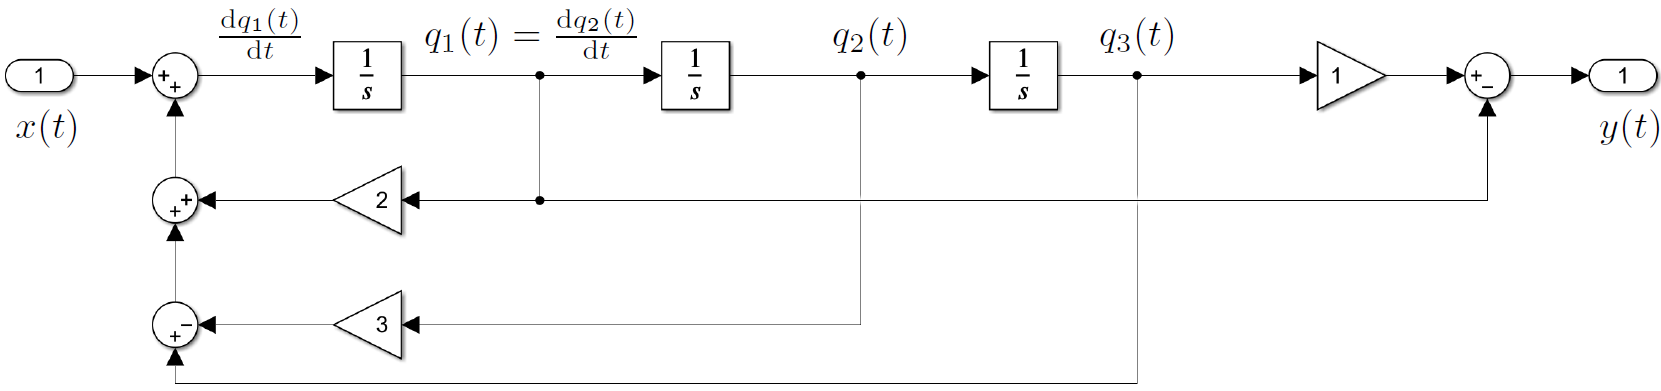
\includegraphics[width=\columnwidth]{images/beispiel_zrd_aus_sfd.png}

\begin{empheq}[box=\fbox] {align*}
    \underbrace{ \begin{bmatrix} \dot{q}_1(t) \\ \dot{q}_2(t) \\ \dot{q}_3(t) \end{bmatrix} }_{\underline{\dot{q}}(t)} &= 
    \underbrace{ \begin{bmatrix} 2 & -3 & 1 \\ 1 & 0 & 0 \\ 0 & 1 & 0 \end{bmatrix} }_{\bm{A}}
    \cdot \underbrace{ \begin{bmatrix} q_1(t) \\ q_2(t) \\ q_3(t) \end{bmatrix} }_{\underline{q}(t)} 
    + \underbrace{ \begin{bmatrix} 1 \\ 0 \\ 0 \end{bmatrix} }_{\bm{B}} \cdot x(t) \\
    y(t) &= \underbrace{ \begin{bmatrix} -1 & 0 & 1 \end{bmatrix}}_{\bm{C}} 
    \cdot \underbrace{ \begin{bmatrix} q_1(t) \\ q_2(t) \\ q_3(t) \end{bmatrix} }_{\underline{q}(t)} 
    + \underbrace{ \begin{bmatrix} 0 \end{bmatrix} }_{\bm{D}} \cdot x(t)
\end{empheq}


\subsection{Zustandsraumdarstellung (ZRD) im Laplace-Bereich}{264}

\begin{minipage}[c]{0.44\columnwidth}
    \vspace{-0.3cm}
    
    \begin{empheq}[box=\fbox] {align*}
        s \underline{X}(s) - x(0) &= \bm{A} \underline{X}(s) + \bm{B} \underline{U}(s) \\
        \underline{Y}(s) &= \bm{C} \underline{X}(s) + \bm{D} \underline{U}(s)
    \end{empheq}

    \begin{tabular}{ll@{}}
        $\underline{U}(s)$   & Eingangsvektor ($m$ Zeilen) \\
        $\underline{X}(s)$   & Zustandsvektor ($n$ Zeilen) \\
        $\underline{Y}(s)$   & Ausgangsvektor ($k$ Zeilen) \\
        $\bm{I}$             & Einheitsmatrix \\
        $\bm{H(s)}$          & Übertragungsmatrix ($k \times m$)\\
    \end{tabular}

\end{minipage}
\hfill
\begin{minipage}[c]{0.54\columnwidth}
    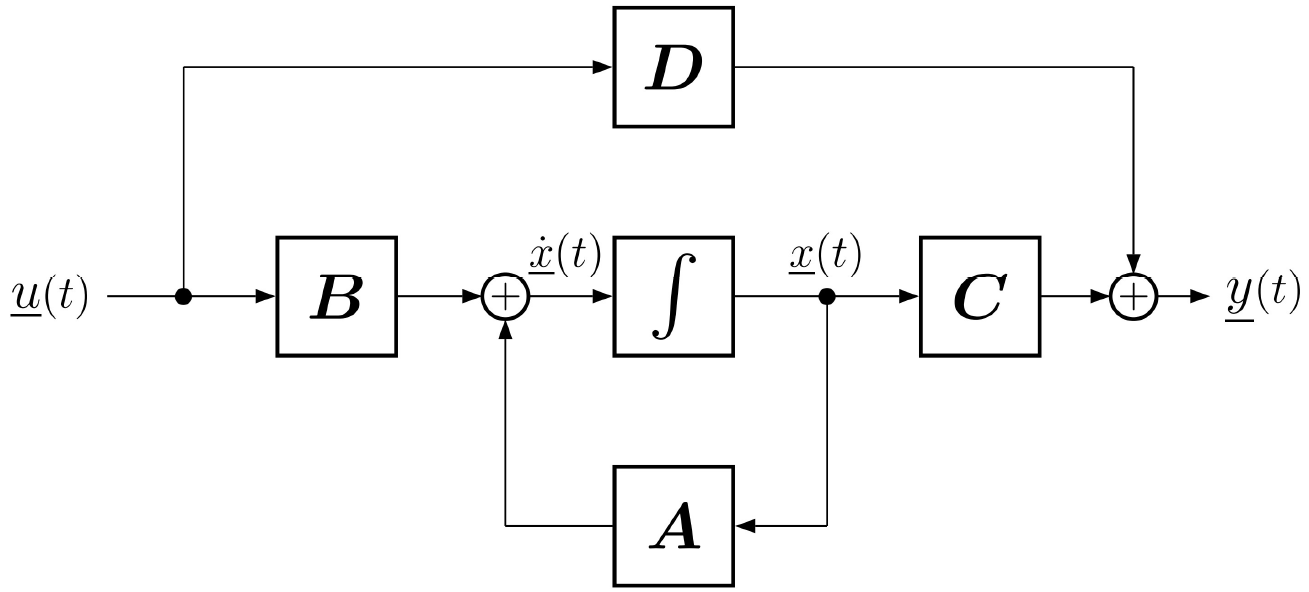
\includegraphics[width=\columnwidth]{images/blockdiagramm_zustandsdarstellung.png}
\end{minipage}

\vspace{0.2cm}
$$ \boxed{ \underline{Y}(s) = \bm{C}(s \bm{I} - \bm{A})^{-1} \underline{x}(0) 
    + \underbrace{(\bm{C}(s \bm{I} - \bm{A})^{-1} \bm{B} + \bm{D} )}_{\bm{H(s)}} \underline{U}(s) } $$

Mit Anfangsbedingungen $x(0) = 0$ ergibt sich folgender Zusammenhang, was der Übertragungsfunktion (UTF) entspricht,
aber im allgemeinen Fall eine \textbf{Matrix} ist.
$$ \boxed{ \underline{Y}(s) = \underbrace{(\bm{C}(s \bm{I} - \bm{A})^{-1} \bm{B} + \bm{D} )}_{\bm{H(s)}} \underline{U}(s) } $$

\textbf{Hinweis:} Aus einem Signalflussdiagramm (SFD) ist es meist sehr einfach, die gesuchten Grössen der ZRD zu finden.


\subsubsection{Übertragungsmatrix und Übertragungsfunktion}{266}

\begin{minipage}[t]{0.48\columnwidth}
    \begin{center}
        \textbf{\myul{Übertragungsmatrix}}
    \end{center}
    \begin{itemize}
        \item MIMO-Systeme
        \item Beschreibung in Matritzenform
            $$ Y(s) = \bm{H(s)} \cdot U(s) $$
        \item  $H(s)$ hat gleiche Grösse (Dimensionen) wie Durchgangsmatrix $\bm{D}$
    \end{itemize}
\end{minipage}
\hfill
\begin{minipage}[t]{0.48\columnwidth}
    \begin{center}
        \textbf{\myul{Übertragungsfunktion}}
    \end{center}
        \begin{itemize}
            \item SISO-Systeme
            \item Matrix-Form wird zu 'normaler' Gleichung
            $$ Y(s) = H(s) \cdot U(s) $$
        \end{itemize}
\end{minipage}


\subsection{Ordnung eines Systems}{256}

Die \textbf{Ordnung} eines Systems definiert die \textbf{kleinste Anzahl von Zustandsgrössen} $x(t)$.
Äquivalent dazu kann die Ordnung eines Systems auch als die \textbf{Anzahl der unabhängigen Energiespeicher} definiert werden.


\subsection{ZRD mit Matlab}

$$ H(s) = \frac{b_i s^i + b_{i-1} s^{i-1} \cdots b_1 s^1 + b_0}{a_i s^i + a_{i-1} s^{i-1} \cdots a_1 s^1 + a_0} $$
\lstinputlisting{snippets/zrd_frequenzbereich.m}


\subsection{Äquivalente Zustandsraumdarstellung (ZRD)}{257}
\label{Äquivalente ZRD}

Mit einer \textbf{Transformationsmatrix} $\bm{T}$ ($n \times n$-Matrix, nicht singulär, $\bm{T T^{-1} = I = T^{-1} T}$) kann man 
\textbf{verschiedenste Zustandsgrössen und Zustandsraumdarstellungen} erhalten, die aber alle ein 
\textbf{identisches Systemverhalten} aufweisen. \\
% Somit kann eine ZRD durch \textbf{verschiedene Schaltungen} realisiert werden, solange diese Schaltungen die 
% \textbf{gleiche Übertragungsfunktion} liefern!

\begin{minipage}[c]{0.4\columnwidth}
    \vspace{-0.3cm}
    
    \begin{empheq}[box=\fbox] {align*}
        \underline{\dot{\xi}}(t) &= \overbrace{ \bm{ T A T}^{-1}}^{\bm{\hat{A}}} \underline{\xi}(t) + \overbrace{\bm{T B}}^{\bm{\hat{B}}}  \underline{u}(t) \\
        \underline{y}(t) &= \underbrace{\bm{C T}^{-1}}_{\bm{\hat{C}}} \underline{\xi}(t) + \underbrace{\bm{D}}_{\bm{\hat{D}}} \underline{u}(t)
    \end{empheq}
\end{minipage}
\hfill
\begin{minipage}[c]{0.58\columnwidth}
    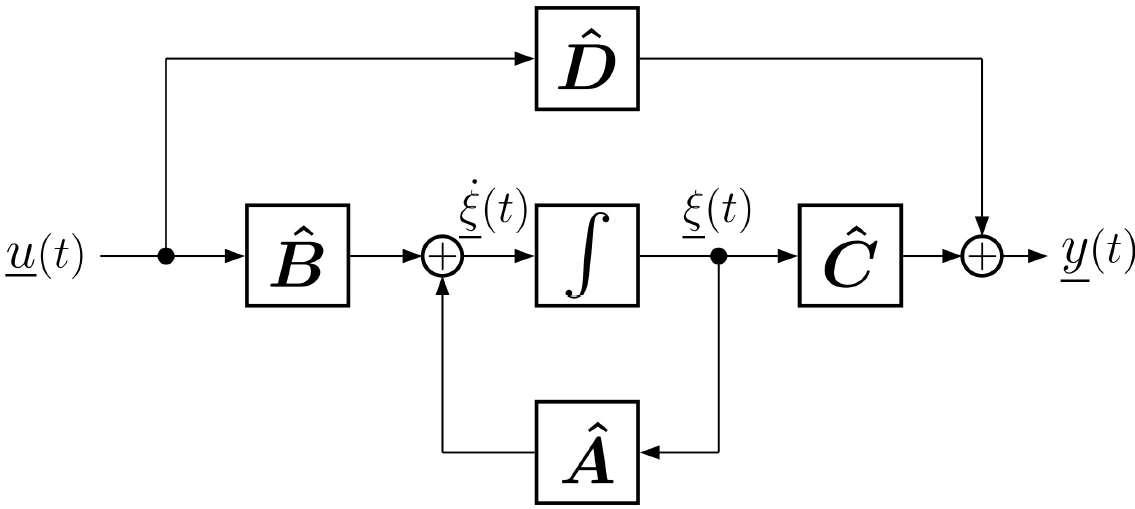
\includegraphics[width=\columnwidth]{images/aequivalente_zrd.png}
\end{minipage}

Die obige ZRD ist \textbf{äquivalent} zur ZRD aus Abschnitt ~\ref{ZRD Zeitbereich} bezüglich $\underline{y}(t)$ und $\underline{u}(t)$.
Die bedeutet, dass die \textbf{Zustandsgrössen} $\underline{\xi}(t)$ und $\underline{x}(t)$ \textbf{willkürlich} gewählt 
werden können, solange $\bm{T}$ nicht singulär ist (Determinante von $\bm{T} \neq 0$) \\

Physikalisch sinnvolle Zustandsgrössen sind:
\begin{itemize}
    \item Spannungen über Kapazitäten
    \item Ströme durch Induktivitäten
\end{itemize}


\subsection[Matrix A diagonalisieren]{Matrix $\bm{A}$ diagonalisieren}

Oft wird die \textbf{Systemmatrix} $\bm{A}$ diagonalisiert, um \textbf{entkoppelte Zustände} zu erhalten. Anstelle der Matrix
$\bm{\hat{A}} = \bm{ T A T}^{-1}$ wird dann üblicherweise $\bm{A_{\rm diag}}$ verwendet.

\begin{tabular}{ll}
    $\lambda_i$                         & Eigenwerte der Matrix $\bm{A}$ \\
    $\vec{v}_i$                         & Eigenvektoren der Matrix $\bm{A}$ \\
    $\bm{V}$                            & Matrix mit Eigenvektoren von $\bm{A}$ \\
    $\bm{A_{\rm diag}} = \bm{\Lambda}$  & Diagonalisierte Matix $\bm{A}$ mit Eigenwerten $\lambda_i$ auf Diagonale \\
    $\bm{T}$                            & Transformationsmatrix 
\end{tabular}

\begin{minipage}[c]{0.48\columnwidth}
    $$ \boxed{\bm{A_{\rm diag}} = \bm{\Lambda} =  \bm{V}^{-1} \cdot \bm{A} \cdot \bm V} $$
\end{minipage}
\hfill
\begin{minipage}[c]{0.48\columnwidth}
    \begin{empheq}[box=\fbox] {align*}
        \bm{T} &= \bm{V}^{-1} \\
        \bm{T}^{-1} &= \bm{V} 
    \end{empheq}
\end{minipage}


\subsubsection{Vorgehen Matrix diagonalisieren}

\begin{outline}
    \1 Ansatz: $ \bm{A} \cdot \vec{v} = \lambda \cdot \vec{v}$ \textrightarrow\ $(\bm{A} - \lambda \bm{I}) \cdot \vec{v} = \vec{0}$ bzw. 
        $(\lambda \bm{I} - \bm{A}) \cdot \vec{v} = \vec{0}$
    \1 Determinante des charakteristischen Polynoms Null setzen: $\abs{\lambda \bm{I} - \bm{A}} = 0$ \\
        \textrightarrow\ Eigenwerte $\lambda_i$ 
    \1 Für jeden gefundenen Eigenwert müssen Eigenvektoren $\vec{v}_i$ gefunden werden:
        \2 Eigenwert $\lambda_i$ in Gleichungssystem $(\lambda_i \bm{I} - \bm{A}) \cdot \vec{v}_i = \vec{0}$ einsetzen
        \2 Einen Wert von $\vec{v}_i = 1$ wählen und Eigenvektor $\vec{v}_i$ als Spaltenvektor schreiben
    \1 Matrix $\bm{V}$ aus Eigenvektoren 'zusammenbauen'
    \1 Matrix $\bm{\Lambda}$ 'zusammenbauen', indem man Eigenwerte $\lambda_i$ auf Diagonale schreibt
\end{outline}


\subsubsection{Entkoppeltes vs. nicht-entkoppeltes System}

\begin{minipage}[t]{0.4\columnwidth}
    \begin{center}
        \myul{\textbf{Nicht-entkoppeltes System}}
    \end{center}
    $$ \bm{A} = \begin{bmatrix*}[r] -2 & 7 \\ -1 & 6 \end{bmatrix*} $$
    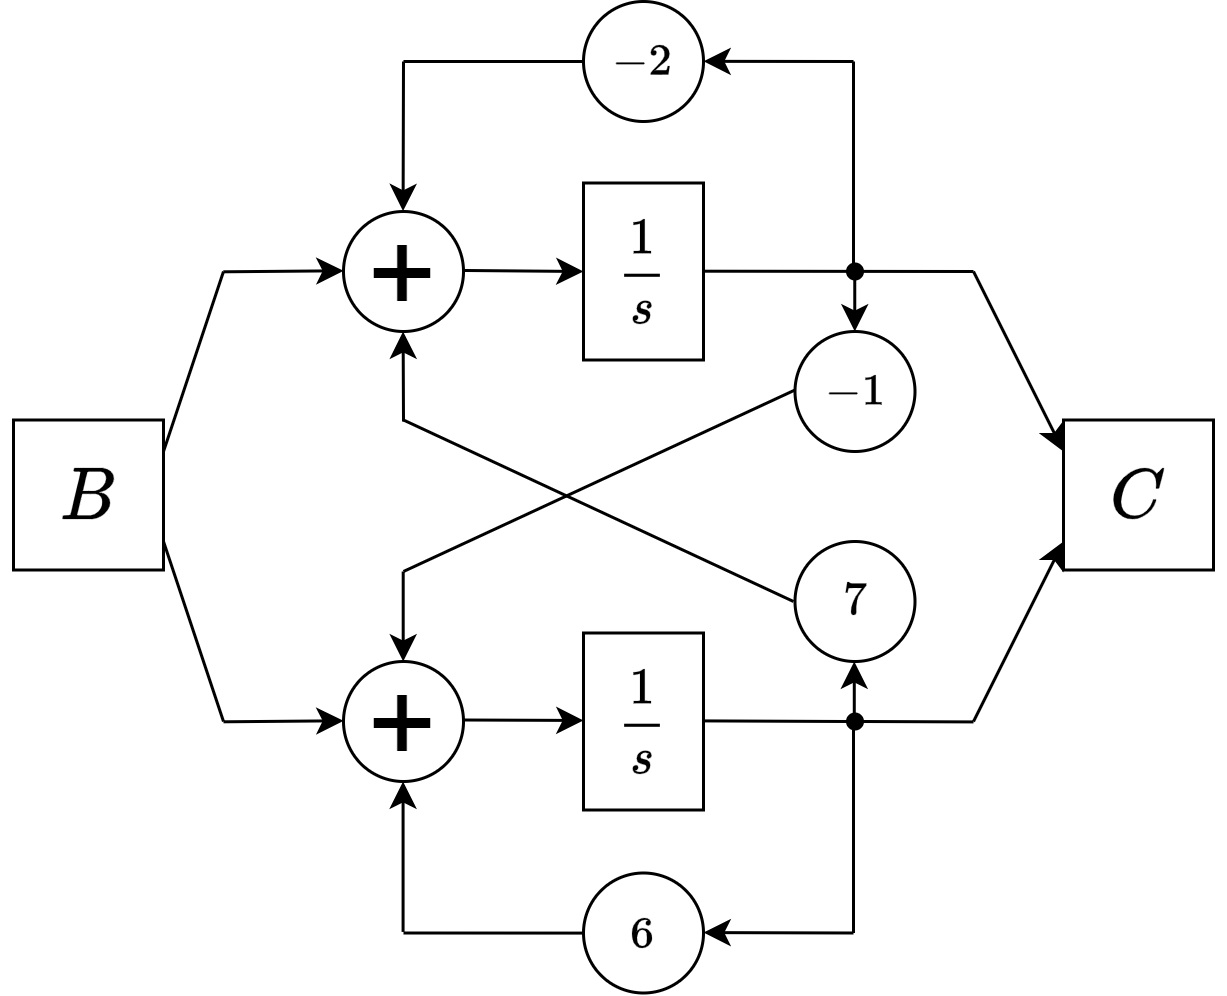
\includegraphics[width=\columnwidth]{images/kreuzform.png}
\end{minipage}
\hfill
\begin{minipage}[t]{0.48\columnwidth}
    \begin{center}
        \myul{\textbf{Entkoppeltes System}}
    \end{center}
    $$ \bm{\hat{A}} = \bm{A_{\rm diag}} = \begin{bmatrix*}[r] -1 & 0 \\ 0 & 5 \end{bmatrix*} $$
    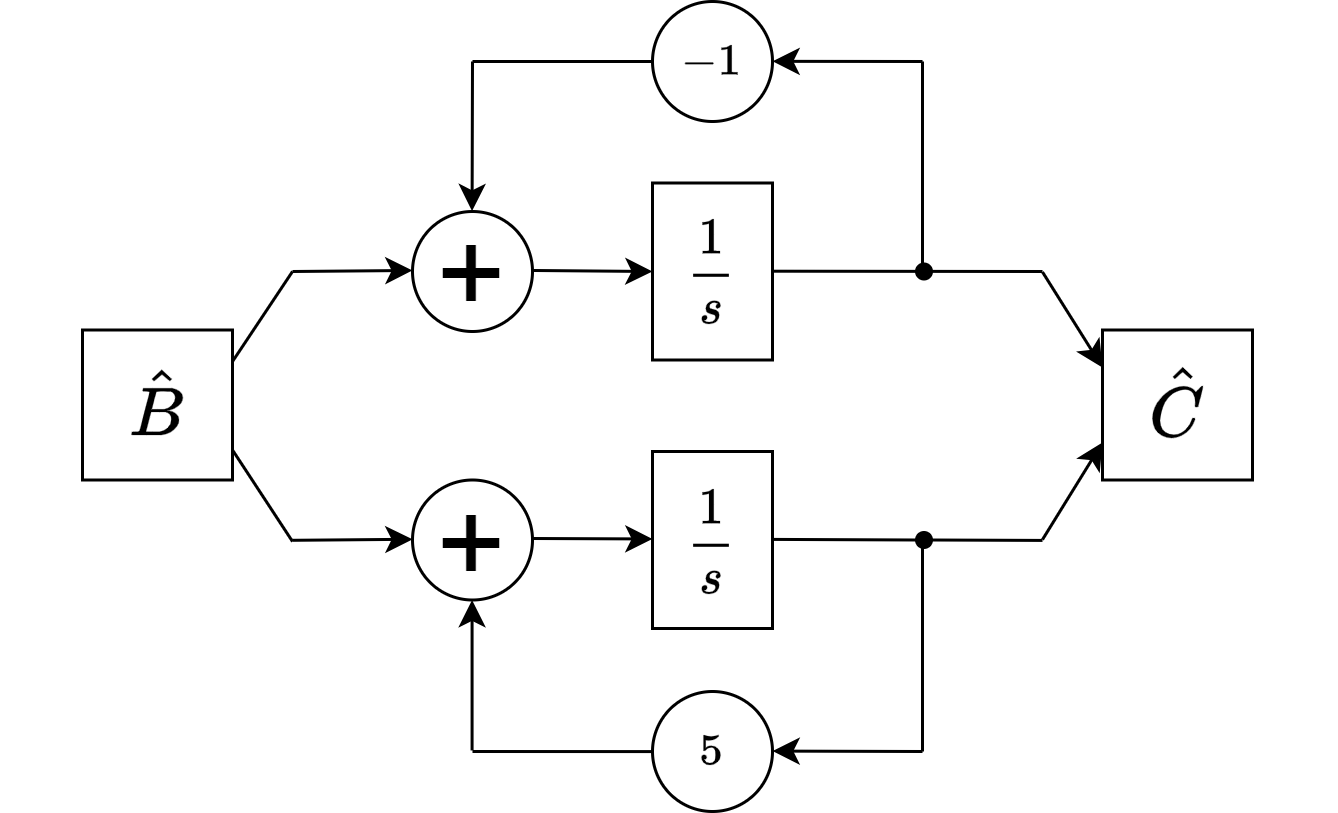
\includegraphics[width=\columnwidth]{images/parallelform.png}
\end{minipage}


\subsection{Einschub -- Lineare Algebra: 2x2 Matrix invertieren}

\begin{minipage}[b]{0.33\columnwidth}
    $$ \bm{A} = 
    \begin{bmatrix*}[r]
        a & b \\
        c & d 
    \end{bmatrix*} $$
\end{minipage}
\hfill
\begin{minipage}[b]{0.66\columnwidth}
    $$ \bm{A}^{-1} = \frac{1}{\det(\bm{A})} \cdot 
    \begin{bmatrix*}[r]
        d & -b \\
        -c & a 
    \end{bmatrix*} \quad \text{ mit } \det(\bm{A}) = ad - bc $$
\end{minipage}


\example{Matrix-Diagonalisierung}{258}

\begin{minipage}[c]{0.25\columnwidth}
    $$ \bm{A} = \begin{bmatrix*}[r]
        -2 & 7 \\
        -1 & 6 
    \end{bmatrix*}$$ 
\end{minipage}
\hfill
\begin{minipage}[c]{0.72\columnwidth}
    $$ \abs{\lambda \bm{I} - \bm{A}} = \begin{vmatrix*}[c]
        \lambda + 2 & -7 \\
        1 & \lambda - 6 
    \end{vmatrix*} = (\lambda + 2) \cdot (\lambda - 6) - 7 \cdot (-1) = 0 $$
\end{minipage}

\textrightarrow\ Mitternachtsformel liefert die Eigenwerte $\lambda_1 = -1$ und $\lambda_2 = 5$

\begin{minipage}[t]{0.56\columnwidth}
    Ersten Eigenwert $\lambda_1 = -1$ in $(\lambda_1 \bm{I} - \bm{A}) \cdot \vec{v}_1 = \vec{0}$ einsetzen
\end{minipage}
\hfill
\begin{minipage}[c]{0.4\columnwidth}
    \begin{align*}
        1 \cdot v_{11} - 7 \cdot v_{21} &= 0 \\
        1 \cdot v_{11} - 7 \cdot v_{21} &= 0 
    \end{align*}
\end{minipage}

\begin{minipage}[c]{0.4\columnwidth}
    Wähle $v_{21} = 1$ \quad \textrightarrow\ $ \vec{v}_1 = \begin{bmatrix*}[r] 7 \\ 1 \end{bmatrix*} $
\end{minipage}
\hfill
\begin{minipage}[c]{0.56\columnwidth}
   Gleichen Vorgehen für zweiten Eigenvektor $\vec{v}_2$
\end{minipage}

\begin{minipage}[c]{0.48\columnwidth}
    $$ \Lambda = \begin{bmatrix} \lambda_1 & 0 \\ 0 & \lambda_2 \end{bmatrix} $$
\end{minipage}
\hfill
\begin{minipage}[c]{0.48\columnwidth}
    $$ \bm{V} = \begin{bmatrix} \vec{v}_1 & \vec{v}_2 \end{bmatrix} = \begin{bmatrix} v_{11} & v_{12} \\ v_{21} & v_{22} \end{bmatrix} $$
\end{minipage}


\subsection{Lösung der ZRD im Zeitbereich}{259-260}
\label{ZRD Lösung Zeitbereich}

Die Zustandsgleichung $\underline{\dot{x}}(t) = \bm{A} \underline{x}(t) + \bm{B} \underline{u}(t)$ ist eine Differentialgleichung.
Sie soll mit dem Ansatz einer Exponentialfunktion gelöst werden. Für Systeme mit nur einem Zustand würde man den Ansatz 
$\underline{x}(t) = e^{at}$ wählen. \\
Da im Allgemeinen Systeme mit mehreren Zuständen betrachtet werden, wird der folgende Ansatz gewählt:

$$ e^{\bm{A} t} = \bm{I} + \bm{A} t + \frac{\bm{A}^2}{2!} t^2 + \cdots + \frac{\bm{A}^k}{k!} t^k + \cdots 
    = \sum\limits_{k=0}^{\infty} \frac{\bm{A}^k t^k}{k!} $$

Der Ansatz ist beschrieben als desser \textbf{Taylor-Reihe.}

Durch einsetzen des Ansatzes in die Zustandsgleichung ergibt sich für den Ausgangsvektor $\underline{y}(t)$ die folgende Lösung
der ZRD im Zeitbereich

$$ \boxed{ \underline{y}(t) = \bm{C} \, \bm{\Phi}(t) \, \underline{x}(0) + 
    \int\limits_0^t \bm{C} \, \bm{\Phi}(t - \tau) \, \bm{B} \, \underline{u}(t) \, \diff \tau + \bm{D} \, \underline{u}(t) } $$

\textbf{Hinweis:} $\bm{\Phi}(t) = e^{\bm{A} t}$ heisst \textbf{Fundamentalmatrix}. 


\subsection{Fundamentalmatrix}{260-263}

Die Fundamentalmatrix (auch Transitionsmatrix genannt) ist definiert als
$$ \boxed{  e^{\bm{A} t} = \bm{\Phi}(t) } $$

Sie wird benötigt, um die Zustandsraumdarstellung im \textbf{Zeitbereich} zu lösen.
Es gibt mehrere Methoden, die quadratische $(n \times n)$ Fundamentalmatrix zu bestimmen


\subsubsection{Methode 1 -- Inverse Laplace-Transformation}

$$ \boxed{ \bm{\Phi}(t) = \mathcal{L}^{-1} \Bigl\{ (s \bm{I} - \bm{A}^{-1})  \Bigr\} } $$


\example{Methode 1 -- Inverse Laplace-Transformation}

Mit der \textbf{Systemmatrix} $\bm{A} = \begin{bmatrix*}[r] -1 & 0 \\ 1 & -2 \end{bmatrix*}$ ergibt sich 
$(s \bm{I} - \bm{A}) = \begin{bmatrix*} s+1 & 0 \\ -1 & s+2 \end{bmatrix*}$

Somit ist $(s \bm{I} - \bm{A})^{-1} = \frac{\begin{bmatrix*} s+1 & 0 \\ -1 & s+2 \end{bmatrix*}}{(s+1)(s+2)} \,
\laplace \, \begin{bmatrix*} e^{-t} & 0 \\ e^{-t} - e^{-2t} & e^{-2t} \end{bmatrix*} = \bm{\Phi}(t)$


\subsubsection{Methode 2 -- Diagonalisierung von $\bm{\Phi}(t) = e^{\bm{A} t}$}

\begin{minipage}[c]{0.6\columnwidth}
    $$ \bm{\Phi}(t) = e^{\bm{A} t} = \underbrace{ 
    \begin{bmatrix*} 
        e^{\lambda_1 t} &                   & \cdots        & 0      \\
                        & e^{\lambda_2 t}   &               & \vdots \\
        \vdots          &                   & \ddots        &        \\
        0               & \cdots            &               & e^{\lambda_n t}
\end{bmatrix*}}_{\bm{\Phi_{\rm diag}(t)}} \cdot \bm{V}^{-1} $$
\end{minipage}
\hfill
\begin{minipage}[c]{0.36\columnwidth}
    Wenn $\bm{A_{\rm diag}} = \bm{V}^{-1} \cdot A \cdot \bm{V}$ ist und $\lambda_i$ die Eigenwerte von $\bm{A}$ sind
\end{minipage}


\subsubsection{Methode 3 -- Spektrale Zerlegung}

\textrightarrow\ Nicht in Vorlesung behandelt


\subsubsection{Methode 4 -- Satz von Cayley-Hamilton}
\textrightarrow\ Nicht in Vorlesung behandelt


\subsubsection{Methode 5 -- Definition der Reihenentwicklung}

% Gemäss Abschnitt ~\ref{ZRD Lösung Zeitbereich} ist die Fundamentalmatrix $\bm{\Phi}(t) = e^{\bm{A} \cdot t}$ als Taylor-Reihe
% definiert.

\begin{minipage}[c]{0.6\columnwidth}
    Die Matrix $\bm{A}$ sei definiert als eine \textbf{Dreiecksmatrix} mit Parameteren $a$ und $c$
\end{minipage}
\hfill
\begin{minipage}[c]{0.38\columnwidth}
    $$ \bm{A} = \begin{bmatrix*} a & 0 \\ 1 & c \end{bmatrix*} $$
\end{minipage}


\begin{minipage}[c]{0.5\columnwidth}
    Die Potenz der Matrix wird berechnet aus
\end{minipage}
\hfill
\begin{minipage}[c]{0.48\columnwidth}
    $$ \bm{A}^k = \begin{bmatrix*} a & 0 \\ 1 & c \end{bmatrix*}^k 
    = \begin{bmatrix*} a^k & 0 \\ \sum\limits_{l=0}^{k-1} a^{k-l-1} c^l  & c^k \end{bmatrix*} $$
\end{minipage}

\example{Methode 5 -- Definition der Reihenentwicklung}

Für $a = 1$ und $c=-1$ ergibt sich für $\bm{A}^k$
$$ \bm{A}^k = \begin{bmatrix*} a & 0 \\ 1 & c \end{bmatrix*}^k 
    = \begin{bmatrix*} \cor{(-1)^k} & 0 \\ \cgn{(-1)^k} - \cvt{(-2)^k} & cbl{(-2)^k} \end{bmatrix*} $$

Die entsprechende Fundamentalmatrix ist mittels Anwendung der Taylor-Reihe somit
$$ e^{\bm{A} t} = \sum\limits_{k=0}^{\infty} \frac{\bm{A}^k t^k}{k!} =
    \begin{bmatrix*} \sum\limits_{k=0}^{\infty} \frac{\cor{(-1)^k}t^k}{k!} & 0 \\ 
    \sum\limits_{k=0}^{\infty} \frac{\cgn{(-1)^k}t^k}{k!} - \sum\limits_{k=0}^{\infty} \frac{\cvt{(-2)^k}t^k}{k!} 
    & \sum\limits_{k=0}^{\infty} \frac{\cbl{(-2)^k}t^k}{k!} \end{bmatrix*} 
    = \begin{bmatrix*} e^{\cor{-t}} & 0 \\ e^{\cgn{-t}} - e^{\cvt{-2t}} & e^{\cbl{-2t}} \end{bmatrix*} $$


\subsubsection{Eigenschaften der Fundamentalmatrix $\bm{\Phi(t) = e^{\bm{A} t}$}}

\begin{tabular}{l c l}
    \toprule
    $\bm{\Phi}(0) = \bm{I} $            & & $e^{\bm{A} \cdot 0} = \bm{I}$ \\
    \midrule
    $\bm{\Phi}^{-1}(t) = \bm{\Phi}(-t)$ & & $\big( e^{\bm{A} \cdot t} \big)^{-1} = e^{- \bm{A} \cdot t}$ \\
    \midrule
    $\bm{\Phi}^k(t) = \bm{\Phi}(kt)$    & & $\big( e^{\bm{A} \cdot t} \big)^k = e^{\bm{A} \cdot k \cdot t}$ \\
    \midrule
    $\bm{\Phi}(t_1) \cdot \bm{\Phi}(t_2) = \bm{\Phi}(t_1 + t_2)$                & & $e^{\bm{A} \cdot t_1} \cdot e^{\bm{A} \cdot t_2} = e^{\bm{A} (t_1 + t_2)}$ \\
    \midrule
    $\bm{\Phi}(t_2 - t_1) \cdot \bm{\Phi}(t_1 - t_0) = \bm{\Phi}(t_2 - t_0)$    & & $e^{\bm{A} (t_2 - t_1)} \cdot e^{\bm{A} (t_1 - t_0)} = e^{\bm{A} (t_2 - t_0)}$ \\
    \bottomrule
\end{tabular}

\vspace{0.2cm}
\textbf{Hinweis:} ($\bm{\Phi}(t)$ ist stets invertierbar)


\subsubsection{Fundamentalmatrix in Matlab}

\lstinputlisting{snippets/fundamentalmatrix.m}

% --------------------------------------------------------------------------------------------------

\subsection{Lösung der ZRD im Zeitbereich -- SISO-Systeme}{263}

Die Impulsantwort $h(t)$ eines SISO-Systems ist gegeben durch

\begin{empheq}[box=\fbox] {align*}
    y(t) &= \bm{C} \bm{\Phi}(t) \bm{B} * u(t) + \bm{D} u(t) = h(t) * u(t) \\
    h(t) &= \bm{C} \bm{\Phi}(t) \bm{B} + \bm{D} \delta(t)
\end{empheq}


\subsection{Stabilität von ZRDs}{275}

Ein LTI-System ist \textbf{asymptotisch stabil}, wenn alle Pole in der linken Halbebene liegen (bzw. einen negativen Realteil haben). \\
Unter Betrachtung der ZRD wird diese Bedingung interpretiert als:
Wenn alle \textbf{Eigenwerte} der \textbf{Systemmatrix} $\bm{A}$ einen \textbf{negativen Realteil} besitzen, ist das System 
\textbf{asymptotisch stabil}.

$$ \boxed{ \abs{\lambda \bm{I} - \bm{A}}  = 0 \quad \rightarrow \forall \lambda \quad \Re{\lambda} < 0 }  $$

\textbf{Achtung: Umgekehrt gilt diese Aussage nicht!} Ein asymptotisch stabiles LTI-System bedeutet \textbf{nicht}, 
dass alle Eigenwerte der Systemmatrix $\bm{A}$ des Systems einen negativen Realteil besitzen. \\
\textrightarrow\ Pol-/Nullstellenkürzungen


\subsection{Beobachtbarkeit und Steuerbarkeit -- Begriffe}{277}

\subsubsection*{Beobachtbarkeit der Zustände}

\begin{itemize}
    \item Ein System ist \textbf{beobachtbar}, wenn wir, gegeben das Eingangssignal $\underline{u}(t)$ und das Ausgangssignal $\underline{y}(t)$,
        über eine endliche Zeitspanne $t_0 \leq t \leq t_1$ die Zustände $\underline{x}(t)$ eindeutig bestimmen können. 
    \item Ein System ist \textbf{nicht beobachtbar}, wenn es Zustände $\underline{x}(t)$ gibt, die \textbf{keinen} Einfluss
        auf die Ausgänge $\underline{y}(t)$ haben. \\   
        \textrightarrow Man kann aus dem Verhalten von $\underline{y}(t)$ \textbf{nicht} auf die Zustände $\underline{x}(t)$ schliessen.
\end{itemize}


\subsubsection*{Steuerbarkeit der Zustände}

\begin{itemize}
    \item Ein System ist \textbf{steuerbar}, wenn es für jeden Anfangszustand $\underline{x}_0$ und jeden Endzustand $\underline{x}_1$
        eine Steuerfunktion $\underline{u}(t)$ gibt, die das System in einer endlichen Zeitspanne $t_0 \leq t \leq t_1$ von
        $\underline{x}_0$ zu $\underline{x}_1$ bringt, d.h. $\underline{x}(t_1) = \underline{x}_1$. 
    \item Ein System ist \textbf{nicht steuerbar}, wenn es Zustände $\underline{x}(t)$ gibt, die nicht von den 
        Eingängen $\underline{u}(t)$ beeinflusst werden. 
\end{itemize}

\vspace{0.2cm}
\textbf{Bemerkungen: }
\begin{itemize}
    \item System ($\bm{A}$, $\bm{B}$, $\bm{C}$, $\bm{D}$) ist bekannt 
    \item Äquivalent reicht es, wenn wir $\underline{x}(0)$ bestimmen können
\end{itemize}
    

\subsection{Steuerbarkeit}{277}

Gemäss der äquivalenten ZRD-Darstellung (siehe Abschnitt~\ref{Äquivalente ZRD}) werden die Matritzen $\bm{\hat{A}}$,
$\bm{\hat{B}}$, $\bm{\hat{C}}$ und $\bm{\hat{D}}$ mit einer Matrix $\bm{V}$ diagonalisert, sodass 
$\bm{\hat{A}} = \bm{A_{\rm diag}} = \bm{V^{-1} A V}$, $\bm{\hat{B}} = \bm{V^{-1} B}$, 
$\bm{\hat{C}} = \bm{C V}$ und $\bm{\hat{D}} = \bm{D}$

\vspace{0.2cm}

\fbox{\parbox{0.95\columnwidth}{
Ein \textbf{SISO-System} mit \textbf{einfachen Eigenwerten} ist genau dann \textbf{vollständig steuerbar}, wenn nach der
Transformation auf \textbf{Diagonalform} bzw. Parallelform ($\bm{A_{\rm diag}} = \bm{\hat{A}} =  \bm{V^{-1} A V}$), 
\textbf{alle} Elemente von $\bm{\hat{B}} = \bm{V^{-1} B}$ \textbf{ungleich Null} sind.
}}
\vspace{0.2cm}

\fbox{\parbox{0.95\columnwidth}{
Ein \textbf{MIMO-System} ($m > 1$) mit \textbf{einfachen Eigenwerten} ist genau dann \textbf{vollständig steuerbar}, wenn nach der
Transformation auf \textbf{Parallelform} ($\bm{A_{\rm diag}} = \bm{\hat{A}} =  \bm{V^{-1} A V}$), in \textbf{jeder Zeile} von 
$\bm{\hat{B}} = \bm{V^{-1} B}$ \textbf{mindestens ein} Element \textbf{ungleich Null} ist.
}}


\subsubsection{Steuerbarkeitsmatrix}

Ein System ist \textbf{vollständig steuerbar}, wenn
\begin{itemize}
    \item Der \textbf{Rang} der Steuerbarkeitsmatrix gleich der \textbf{Ordnung} $n$ des Systems
    \item Falls nur \textbf{ein Eingang} ($m = 1$): Die \textbf{Determinante} von $\bm{Q}_{\rm Steuerbarkeit}$ 
        \textbf{ungleich Null ist}
\end{itemize}

\begin{minipage}[c]{0.6\columnwidth}
    $$ \boxed{ \bm{Q}_{\rm Steuerbarkeit} = 
    \begin{bmatrix}
        \bm{B} & \bm{A B} & \bm{A^2 B} & \cdots & \bm{A^{n-1} B} 
    \end{bmatrix} } $$
\end{minipage}
\hfill
\begin{minipage}[c]{0.38\columnwidth}
    Dimension: $n \times n \cdot m$
\end{minipage}


\begin{minipage}[c]{0.48\columnwidth}
    \begin{tabular}{ll}
        $\bm{A}$    & Systemmatrix ($n \times n$) \\
        $\bm{B}$    & Eingangsmatrix ($n \times m$) \\
    \end{tabular}
\end{minipage}
\hfill
\begin{minipage}[c]{0.48\columnwidth}
    \begin{tabular}{ll}
        $n$         & Zustände \\
        $m$         & Eingänge \\
    \end{tabular}
\end{minipage}


\subsubsection*{Steuerbarkeitsmatrix in Matlab}

\lstinputlisting{snippets/steuerbarkeitsmatrix.m}


\subsection{Beobachtbarkeit}{278}

Gemäss der äquivalenten ZRD-Darstellung (siehe Abschnitt~\ref{Äquivalente ZRD}) werden die Matritzen $\bm{\hat{A}}$,
$\bm{\hat{B}}$, $\bm{\hat{C}}$ und $\bm{\hat{D}}$ mit einer Matrix $\bm{V}$ diagonalisert, sodass 
$\bm{\hat{A}} = \bm{A_{\rm diag}} = \bm{V^{-1} A V}$, $\bm{\hat{B}} = \bm{V^{-1} B}$, 
$\bm{\hat{C}} = \bm{C V}$ und $\bm{\hat{D}} = \bm{D}$

\vspace{0.2cm}

\fbox{\parbox{0.95\columnwidth}{
Ein \textbf{SISO-System} mit \textbf{einfachen Eigenwerten} ist genau dann \textbf{vollständig beobachtbar}, wenn nach der
Transformation auf \textbf{Diagonalform} bzw. Parallelform ($\bm{A_{\rm diag}} = \bm{\hat{A}} =  \bm{V^{-1} A V}$), 
\textbf{alle} Elemente von $\bm{\hat{C}} = \bm{C V}$ \textbf{ungleich Null} sind.
}}
\vspace{0.2cm}

\fbox{\parbox{0.95\columnwidth}{
Ein \textbf{MIMO-System} ($m > 1$) mit \textbf{einfachen Eigenwerten} ist genau dann \textbf{vollständig beobachtbar}, wenn nach der
Transformation auf \textbf{Parallelform} ($\bm{A_{\rm diag}} = \bm{\hat{A}} =  \bm{V^{-1} A V}$), in \textbf{jeder Spalte} von 
$\bm{\hat{C}} = \bm{C V}$ \textbf{mindestens ein} Element \textbf{ungleich Null} ist.
}}


\subsubsection{Beobachtbarkeitsmatrix}

Ein System ist \textbf{vollständig beobachtbar}, wenn
\begin{itemize}
    \item Der \textbf{Rang} der Beobachtbarkeitsmatrix gleich der \textbf{Ordnung} $n$ des Systems
    \item Falls nur \textbf{ein Eingang} ($m = 1$): Die \textbf{Determinante} von $\bm{Q}_{\rm Beobachtbarkeit}$ 
        \textbf{ungleich Null ist}
\end{itemize}

\begin{minipage}[c]{0.4\columnwidth}
    $$ \boxed{ \bm{Q}_{\rm Beobachtbarkeit} = 
    \begin{bmatrix}
        \bm{C} \\ \bm{C A} \\ \bm{C A^2} \\ \vdots \\ \bm{C A^{n-1}} 
    \end{bmatrix} } $$
\end{minipage}
\hfill
\begin{minipage}[c]{0.58\columnwidth}
    \begin{tabular}{ll}
        Dimension:  & $k \cdot n \times n$ \\
        $\bm{A}$    & Systemmatrix ($n \times n$) \\
        $\bm{C}$    & Beobachtungsmatrix ($k \times m$) \\
        $n$         & Zustände \\
        $m$         & Eingänge \\
        $k$         & Ausgänge 
    \end{tabular}
\end{minipage}


\subsubsection*{Beobachtbarkeitsmatrix in Matlab}

\lstinputlisting{snippets/beobachtbarkeitsmatrix.m}


% \subsection{Ausgangssteuerbarkeit}{280-281}
% nicht behandelt 

% \subsubsection{Ausgangssteuerbarkeitsmatrix}
% nicht behandelt

% \vfill\null
% \columnbreak

\subsection{Standardformen der ZRD}{267}

Die allgemeine Differentialgleichung von SISO-Systemen der Form

$$ a_n \frac{\diff^n y}{\diff t^n} + a_{n-1} \frac{\diff^{n-1} y}{\diff t^{n-1}} + \cdots + a_1 \frac{\diff y}{\diff t} + a_0 y =
    b_m \frac{\diff^m u}{\diff t^m} + b_{m-1} \frac{\diff^{m-1} u}{\diff t^{m-1}} + \cdots + b_1 \frac{\diff u}{\diff t} + b_0 u  $$

ergibt mit der Laplace-Transformation und mit $m \leq n$
$$ \boxed{ H(s) = \frac{Y(s)}{U(s)} = \frac{b_m s^m + b_{m-1} s^{m-1} + \cdots + b_1 s + b_0}
{a_n s^n + a_{n-1} s^{n-1} + \cdots + a_1 s + a_0} }$$

Diese UTF $H(s)$ kann mit verschiedenen ZRDs (\textbf{Normalformen}) abgebildet werden. \\
\cbl{\textbf{Wichtig:} Für alle folgenden Normalformen werden die Zustände $x_i$ im blockdiagramm
\textbf{unmittelbar nach den Integratoren} verwendet.}


\subsubsection{Regelungsnormalform}{267-268}

Die Regelungsnormalform kann \textbf{direkt aus der UTF} $H(s)$ aufgestellt werden.

Für $m = n$ gilt sieht die Regelungsnormalform folgendermassen aus:
\begin{empheq}[box=\fbox] {align*}
    \begin{bmatrix} \dot{x}_1(t) \\ \dot{x}_2(t) \\ \vdots \\ \dot{x}_{n-1}(t) \\ \dot{x}_n(t)  \end{bmatrix} &= 
    \begin{bmatrix} 
        0       & 1         & 0         & \cdots    & 0     \\
        0       & 0         & 1         & \cdots    & 0     \\
        \vdots  & \vdots    & \vdots    & \ddots    & \vdots\\
        0       & 0         & 0         & \cdots    & 1     \\
        -a_0    & -a_1      & -a_2      & \cdots    & -a_{n-1} 
    \end{bmatrix}
    \cdot
    \begin{bmatrix} x_1(t) \\ x_2(t) \\ \vdots \\ x_{n-1}(t) \\ x_n(t) \end{bmatrix}
    + 
    \begin{bmatrix} 0 \\ 0 \\ \vdots \\ 0 \\ 1 \end{bmatrix} 
    \cdot u(t) \\
    y(t) &= \begin{bmatrix} b_0 - a_0 b_n & b_1 - a_1 b_n & \cdots& b_{n-1} - a_{n-1} b_n \end{bmatrix}
    \cdot
    \begin{bmatrix} x_1(t) \\ x_2(t) \\ \vdots \\ x_{n-1}(t) \\ x_n(t) \end{bmatrix}
    + \begin{bmatrix} b_n \end{bmatrix} \cdot u(t)
\end{empheq}

In den meisten Fällen ist $m < n$ und die \textbf{Ausgangsgleichung} vereinfacht sich zu:
\begin{empheq}[box=\fbox] {align*}
    y(t) &= \begin{bmatrix} b_0 &  b_1 & \cdots & b_m & 0 & \cdots & 0 \end{bmatrix}
    \cdot
    \begin{bmatrix} x_1(t) \\ x_2(t) \\ \vdots \\ x_{n-1}(t) \\ x_n(t) \end{bmatrix}
    + \begin{bmatrix} 0 \end{bmatrix} \cdot u(t)
\end{empheq}


% \subsubsection{Alternative Regelungsnormalform}{268}
% nicht behandelt


\subsubsection{Beobachtungsnormalform}{269-270}

Ein System, welches in Beobachtungsnormalform dargestellt werden kann, ist \textbf{beobachtbar!}
ür $m = n$ gilt sieht die Regelungsnormalform folgendermassen aus:
\begin{empheq}[box=\fbox] {align*}
    \begin{bmatrix} \dot{x}_1(t) \\ \dot{x}_2(t) \\ \vdots \\ \dot{x}_{n-1}(t) \\ \dot{x}_n(t)  \end{bmatrix} &= 
    \begin{bmatrix} 
        0       & 0         & 0         & \cdots    & -a_0  \\
        1       & 0         & 0         & \cdots    & -a_1  \\
        0       & 1         & 0         & \cdots    & -a_2  \\
        \vdots  & \vdots    & \ddots    & 0         & \vdots\\
        0       & 0         & \cdots    & 1         & -a_{n-1} 
    \end{bmatrix}
    \cdot
    \begin{bmatrix} x_1(t) \\ x_2(t) \\ \vdots \\ x_{n-1}(t) \\ x_n(t) \end{bmatrix}
    + 
    \begin{bmatrix} b_0 - a_0 b_n \\ b_1 - a_1 b_n \\ b_2 - a_2 b_n \\ \vdots \\ b_{n-1} - a_{n-1} b_n \end{bmatrix} 
    \cdot u(t) \\
    y(t) &= \begin{bmatrix} 0 & 0 & \cdots & 1 \end{bmatrix}
    \cdot
    \begin{bmatrix} x_1(t) \\ x_2(t) \\ \vdots \\ x_{n-1}(t) \\ x_n(t) \end{bmatrix}
    + \begin{bmatrix} b_n \end{bmatrix} \cdot u(t)
\end{empheq}

In den meisten Fällen ist $m < n$ und die \textbf{Zustandsgleichung} vereinfacht sich zu:
\begin{empheq}[box=\fbox] {align*}
    \begin{bmatrix} \dot{x}_1(t) \\ \dot{x}_2(t) \\ \vdots \\ \dot{x}_{n-1}(t) \\ \dot{x}_n(t)  \end{bmatrix} &= 
    \begin{bmatrix} 
        0       & 0         & 0         & \cdots    & -a_0  \\
        1       & 0         & 0         & \cdots    & -a_1  \\
        0       & 1         & 0         & \cdots    & -a_2  \\
        \vdots  & \vdots    & \ddots    & 0         & \vdots\\
        0       & 0         & \cdots    & 1         & -a_{n-1} 
    \end{bmatrix}
    \cdot
    \begin{bmatrix} x_1(t) \\ x_2(t) \\ \vdots \\ x_{n-1}(t) \\ x_n(t) \end{bmatrix}
    + 
    \begin{bmatrix} b_0  \\ b_1 \\ b_2 \\ \vdots \\ b_{n-1} \end{bmatrix} 
    \cdot u(t) \\
\end{empheq}


\subsubsection{Regelungsnormalform $\Leftrightarrow$ Beobachtungsnormalform}

Die beiden Formen sind \textbf{dual} und weisen folgende Zusammenhänge auf (\textbf{Transposition}):

\begin{itemize}
    \item $\bm{A}$ ist an der Hauptdiagonalen gespiegelt 
    \item $\bm{B}$ und $\bm{C}$ sind vertauscht
    \item $\bm{D}$ bleibt gleich
\end{itemize}


% \subsubsection{Alternative Beobachtungsnormalform}{270}
% nicht behandelt


\subsubsection{Jordan-Normalform}{271-273}

Die UTF wird mittels einer \textbf{Partialbruchzerlegung} dargestellt. Die Parameter der Partialbruchzerlegung können dann
direkt in die Matrix $A = A_{\rm diag}$ eingetragen werden.
$$ H(s) = \frac{Y(s)}{U(s)} = \frac{b_m s^m + b_{m-1} s^{m-1} + \cdots + b_1 s + b_0}
{s^n + a_{n-1} s^{n-1} + \cdots + a_1 s + a_0} = b_n + \frac{\alpha_1}{s - p_1} + \frac{\alpha_2}{s - p_2} + \ldots + \frac{\alpha_n}{s - p_n}$$

\vspace{0.2cm}
Die Diagronalform für \textbf{einfache, reelle Pole} mit $m = n$ ist:
\begin{empheq}[box=\fbox] {align*}
    \begin{bmatrix} \dot{x}_1(t) \\ \dot{x}_2(t) \\ \vdots \\ \dot{x}_{n-1}(t) \\ \dot{x}_n(t)  \end{bmatrix} &= 
    \begin{bmatrix} 
        p_1     & 0         & 0         & \cdots    & 0  \\
        0       & p_2       & 0         & \cdots    & 0  \\
        0       & 0         & p_3       & \cdots    & 0  \\
        \vdots  & \vdots    & \ddots    & P_{n-1}  & \vdots\\
        0       & 0         & \cdots    & 0         & p_n
    \end{bmatrix}
    \cdot
    \begin{bmatrix} x_1(t) \\ x_2(t) \\ \vdots \\ x_{n-1}(t) \\ x_n(t) \end{bmatrix}
    + 
    \begin{bmatrix} 1 \\ 1 \\ 1\\ \vdots \\ 1 \end{bmatrix} 
    \cdot u(t) \\
    y(t) &= \begin{bmatrix} \alpha_1 & \alpha_2 & \cdots & \alpha_n \end{bmatrix}
    \cdot
    \begin{bmatrix} x_1(t) \\ x_2(t) \\ \vdots \\ x_{n-1}(t) \\ x_n(t) \end{bmatrix}
    + \begin{bmatrix} b_n \end{bmatrix} \cdot u(t)
\end{empheq}

\textbf{Hinweis:} Mit $m < n$ vereinfacht sich die \textbf{Ausgangsgleichung} zu:
\begin{empheq}[box=\fbox] {align*}
    y(t) &= \begin{bmatrix} \alpha_1 & \alpha_2 & \cdots & \alpha_n \end{bmatrix}
    \cdot
    \begin{bmatrix} x_1(t) \\ x_2(t) \\ \vdots \\ x_{n-1}(t) \\ x_n(t) \end{bmatrix}
    + \begin{bmatrix} 0 \end{bmatrix} \cdot u(t)
\end{empheq}


\subsubsection{Diagonalform}{271-273}

Eine weitere Darstellungsform der Diagonalform ergibt sich mittels \textbf{Transposition} der Jordan-Normalform:

\begin{itemize}
    \item $\bm{A}$ ist an der Hauptdiagonalen gespiegelt (ergibt wiederum $\bm{A}$)
    \item $\bm{B}$ und $\bm{C}$ sind vertauscht
    \item $\bm{D}$ bleibt gleich
\end{itemize}

% \subsubsection{Jorodan-Normalform für mehrfache, reelle Pole}{274}
% nicht behandelt